
%% bare_conf.tex
%% V1.3
%% 2007/01/11
%% by Michael Shell
%% See:
%% http://www.michaelshell.org/
%% for current contact information.
%%
%% This is a skeleton file demonstrating the use of IEEEtran.cls
%% (requires IEEEtran.cls version 1.7 or later) with an IEEE conference paper.
%%
%% Support sites:
%% http://www.michaelshell.org/tex/ieeetran/
%% http://www.ctan.org/tex-archive/macros/latex/contrib/IEEEtran/
%% and
%% http://www.ieee.org/

\documentclass[10pt, conference]{IEEEtran}

\usepackage{booktabs}
\usepackage{cite}
\usepackage{color}
\usepackage{enumerate}
\usepackage[utf8]{inputenc}
\usepackage{tikz}
%\usepackage[brazil]{babel}
%\usepackage[cmex10]{amsmath}
%\usepackage{algorithmic}
%\usepackage{array}
%\usepackage{mdwmath}
%\usepackage{mdwtab}
%\usepackage{eqparbox}
%\usepackage[tight,footnotesize]{subfigure}
%\usepackage[caption=false]{caption}
%\usepackage[font=footnotesize]{subfig}
%\usepackage[caption=false,font=footnotesize]{subfig}
%\usepackage{fixltx2e}
%\usepackage{stfloats}
%\usepackage{url}


\newif\ifComments

% To turn comments OFF simply comment out the \Commentstrue line
\Commentstrue

\ifComments
\newcommand{\luiz}[1]{\noindent\textcolor{cyan}{LUIZ: {#1}}}
\newcommand{\mario}[1]{\noindent\textcolor{cyan}{MARIO: {#1}}}
\newcommand{\rem}[1]{\noindent\textcolor{magenta}{REMOVED: {#1}}}
\newcommand{\new}[1]{\noindent\textcolor{blue}{NEW: {#1}}}
\newcommand{\rev}[1]{\noindent\textcolor{red}{REVISE: {#1}}}
\else
\newcommand{\luiz}[1]{}
\newcommand{\mario}[1]{}
\newcommand{\rem}[1]{}
\newcommand{\new}[1]{#1}
\newcommand{\rev}[1]{#1}
\fi

% correct bad hyphenation here
\hyphenation{}
\usetikzlibrary{shapes.geometric, arrows}

\tikzstyle{activity} = [rectangle, rounded corners, minimum width=5cm, minimum 
height=1cm,text centered, draw=black, fill=white]
\tikzstyle{io} = [trapezium, trapezium left angle=70, trapezium right angle=110, minimum width=3cm, minimum height=1cm, text centered, draw=black, fill=blue!30]
\tikzstyle{process} = [rectangle, minimum width=3cm, minimum height=1cm, text centered, text width=3cm, draw=black, fill=orange!30]
\tikzstyle{decision} = [diamond, minimum width=3cm, minimum height=1cm, text centered, draw=black, fill=green!30]
\tikzstyle{arrow} = [thick,->,>=stealth]
\tikzstyle{line} = [draw, -latex']


\begin{document}

\title{Assessment Accuracy of Random Forest Classifier on Imbalanced Data to Predict Change Request Severity Level}

\author{\IEEEauthorblockN{Luiz Alberto Ferreira Gomes}
\IEEEauthorblockA{Software Engineering Departament\\
Pontifical Catholic University of Minas Gerais - PUC MG\\
Poços de Caldas, Brazil\\
luizgomes@pucpcaldas.br}
\and
\IEEEauthorblockN{Mario Lúcio Côrtes}
\IEEEauthorblockA{Institute of Computing\\
State University of Campinas - UNICAMP\\
Campinas, Brasil\\
cortes@ic.unicamp.br}
}

\maketitle

\begin{abstract}
\rem{In the context de Change Request (CR) systems, the severity level of a change request is considered a critical variable in the planning of the software maintenance activities, indicating as soon a CR needs to be fixed. However, the severity level assignment remains a process primarily manual depending on the experience and expertise who has reported the CR. In this paper, we present the preliminary findings of research aim to predict the severity level of a CR by analyzing its long description using text mining and a classifier based on Random Forest algorithm. The results have evidenced that this classifier can predict the severity level will change and whether severity will increase or decrease with reasonable accuracy, around 94,12\% and 93,86\% respectively. However, it has provided poor accuracy (around 67,29\%) to predict the final last severity level in imbalanced data scenario.} \new{In the context de Change Request (CR) systems, the severity level of a change request is considered a critical variable in the planning of the software maintenance activities, indicating how soon a CR needs to be fixed. However, the severity level assignment remains primarily a manual process, mostly depending on the experience and expertise of the person who has reported the CR. In this paper, we present preliminary findings of research aimed to predict the severity level of a CR by analyzing its long description, using text mining and a classifier based on Random Forest algorithm. The results have evidenced that this classifier can predict the severity level will change and whether severity will increase or decrease with good accuracy, around 94,12\% and 93,86\% respectively. However, it has provided poor accuracy (around 67,29\%) to predict the final last severity level in imbalanced data scenario.} \mario{ultima frase: pensar outra abordagem. Está muito negativo. Dizer a mesma coisa de forma positiva. Comparar com a literatura?
e sobre a nova medida? e comparativo com a literatura (no abstract)?}

\end{abstract}

\begin{IEEEkeywords}
software maintenance; change request systems \mario{Ver nome padrao na literatura; nao seria BTS bug tracking system?}; machine learning; random forest.
\end{IEEEkeywords}


% For peer review papers, you can put extra information on the cover
% page as needed:
% \ifCLASSOPTIONpeerreview
% \begin{center} \bfseries EDICS Category: 3-BBND \end{center}
% \fi
%
% For peerreview papers, this IEEEtran command inserts a page break and
% creates the second title. It will be ignored for other modes.
\IEEEpeerreviewmaketitle



\section{Introduction}
Change Request (CR) systems \rem{has been performed a critical} \new{have played a major} role in maintenance process in many software development settings, both in Close Source Software (CSS) and in Open Source Software (OSS) scenarios. Mainly in the latter, which is characterized by the existence of many of users and developers with \rem{distinct expertise levels} \new{different levels of expertise} spread out around the world, who might \rem{register or deal with any amount of} \new{create or be responsible for dealing with several} change requests\cite{Cavalcanti2014}. 

A user interacts with a CR system often through a simple mechanism called CR form. This form enables him to request changes, to report bugs or to ask for support in a software product\cite{Sommerville2010}. Initially, he or she should inform a short description, a long description, a type (e.g. bug, new feature, improvement, and task) and a \new{associated} severity level (e.g. blocker, critical, major, minor and trivial)\rem{ for his or her solicitation} \mario{evite a palavra solicitation}. Subsequently, a development team member will review this request and, case it is not refused for some reason (e.g. request duplication), he or she will complete the information in CR form, indicating, for example, its priority and the person responsible for accomplishing it. \mario{importante usar terminologia e jargao do ramo: acho que aqui nao eh accomplish e sim assigned for the CR; verificar em outros artigos}

The severity level information is recognized as a critical variable in the equation to estimate a prioritization of change request prioritization\cite{Tian2012} \mario{repetido}. Consequently, it can be a decisive factor how soon it needs to be fixed\cite{Lamkanfi2010}. However, the severity level assignment remains a mostly manual process which relies on experience and expertise of the person who has opened the CR \cite{Cavalcanti2014, Tian2012, Lamkanfi2010}. So, it may allow a high degree of subjectivity and, consequently, it may be quite error-prone. 

The number of CR made is frequently very high in large and medium software projects\cite{Lamkanfi2011}. Severity level shifts throughout CR lifecycle (Figure \ref{fig:cr-life-cycle}) could cause substantial impacts on the maintenance activities planning and could drive the development team to solve the least significant change requests before the most important ones. In this scenario, the support of a computational tool to help the user to assign and the development team to verify the CR severity level well desirable.


\begin{enumerate}[RQ 1:]
  \item \textit{Is it possible to predict whether the change request severity degree will shift during its lifecycle?} Based on long description filled by users in CR form, we have investigated if it is possible to predict using a Random Forest classifier, with a high degree of accuracy in an imbalanced data scenario, whether the severity level of the request will be changed.
  \item \textit{Is it possible to predict whether the change request severity level will increase, decrease or remain the same during its lifecycle}? Based on long description filled by users in CR form, this question has enabled us to investigate if it is possible to predict using Random Forest classifier, with a high degree of accuracy in an imbalanced data scenario,  whether the severity of the request will be increased, decreased or remained the same.
  \item \textit{Is it possible to predict the change request severity degree at the end of its lifecycle?} Finally, we have investigated if it is possible to predict using a Random Forest classifier, with a high degree of accuracy in an imbalanced data scenario, the severity level of a request based on the same information used in the two previous questions.
\end{enumerate}


\begin{figure}[hbt!]  
  \centering
  \begin{tikzpicture}[node distance=1.5cm]
    \node (a1) [activity] {Open};
    \node (a2) [activity, below of=a1] {In Progress};
    \node (a3) [activity, below of=a2] {Resolved};
    \node (a4) [activity, below of=a3] {Closed};
    \node (a5) [activity, below of=a4] {Reopened};
    
    \draw [arrow] (a1) -- (a2);
    \draw [arrow] (a2) -- (a3);
    \draw [arrow] (a3) -- (a4);
    \draw [arrow] (a4) -- (a5);
    \draw [arrow] (a5.east)  -- ++(1.5,0) |- (a1.east);
    \draw [arrow] (a3.west)  -- ++(-1.5,0) |- (a5.west);
  \end{tikzpicture}
  \caption{CR life cycle\cite{Sommerville2010}.}
  \label{fig:cr-life-cycle}
\end{figure}
% TODO: Put here CR life cycle figure.

This paper presents the preliminary results of research whose the objective is to implement an automatic mechanism, based on random forest machine algorithm, aim to aid users, developers and managers to assign the CR severity level more accurately. 
The contributions of this work are as follows

\begin{enumerate}
  \item we...
  \item we...
  \item we...
  
\end{enumerate}

The structure of this paper is as follows. In Section 2, we describe some related works. In Section 3, we provide the information background about CR systems, text mining and machine learning techniques necessary to understand our approach. Section 4 describe our work. Findings and discussions are presented in Section 5. Finally, we conclude and discuss future work in Section 6.


\section{Related Works}

Menzies\cite{Menzies2008} have developed a method, named SEVERIS (SEVERity ISsue assessment), for evaluating the severity of changes requests. SEVERIS is based on common text mining techniques (e.g. tokenization, stop word removal, stemming, Tf*Idf and InfoGain) and on the data mining techniques (e.g. RIPPER). The method was applied to five projects managed by the Project and Issue Tracking System (PITS). - an issue tracker system used by NASA.

Lamkanfi et al.\cite{Lamkanfi2010} have developed an approach to predict severity level of a CR based on text mining algorithms (tokenization, stop word removal, stemming) and on the Naïve Bayes machine learning algorithm. They have been validated their approach over from three open source project Mozilla, Eclipse, and GNOME and they accomplished that a training set with approximately 500 change requests per severity degree are enough to predict it with a reasonable accuracy. In another following work, Lamkanfi et al.\cite{Lamkanfi2011}, these authors compared the accrual of four machine-learning algorithms (Naïve Bayes Multinomial, K-Nearest Neighbor, and Support Vector Machine). They have been concluded that Naïve Bayes Multinomial gave superior performance compared to the others proposed algorithms.

Valdivia et al.\cite{ValdiviaGarcia2014} have characterized blocking bugs in six open source projects and proposed a model to predict them. Their model was composed of 14 distinct factors or features (e.g. the textual description, location the bug is found in and the people involved with the bug). Based on these factors they build decision trees for each project to predict whether a bug will be a blocking bug or not. Then, they analyze these decision trees to determine which factors best indicate these blocking bugs. 

\section{BACKGROUND}
In this section, we describe de change request process. Next we explain the common approach to pre-processing textual documents, and lastly, we highlight the Random Forest algorithm to classify and predict the CR severity level.

\subsection{Change Request Systems}
Change Request systems\cite{Pressman2009} are software employed to keep the recording and tracking information of requests for modifications, bug fixes, and support that could occur during the software life cycle. 

Although there is no a common sense regarding the terminology or the amount of information that users must fill in to complete his requisition between popular CR systems (e.g. Bugzilla, Jira, and Redmine)\cite{Tian2012}, typically, they shall fill in a form containing at least the following attributes shown in Table \ref{tab:commom_attributes_cr_form}. 

\begin{table}[!ht]
	% increase table row spacing, adjust to taste
	\renewcommand{\arraystretch}{1.3}
	\caption{Commom attributes in the CR forms.}
	\label{tab:commom_attributes_cr_form}
	\centering
	\begin{tabular}{|l|p{6cm}|}
		\hline
		Type & Type of request (e.g. bug, new feature, improvement, and new feature)\\
		\hline
		Title & Short description of request in one line.\\
		\hline
		Description & Long and detailed description of request in many lines. It could include source code snippets and stack tracing reports.\\
		\hline
		Severity & Level of severity of request (e.g. blocker, critical, major, minor and trivial).\\
		\hline 
	\end{tabular}
\end{table}

Once the request has been registered by the user, the development team will assess it and, if it not canceled for some reason (e.g. duplication), they will complement the information with, for example, the person responsible for handling this request. All these data are stored in a repository, keeping relevant historical data about a particular software.

\subsection{Text Mining}
Text mining is the process to convert unstructured text into a structure suited to analysis\cite{Feldman2007}. It is composed of three basic activities\cite{Williams2011}: tokenization, stop word removal and stemming.

Tokenization is the action to parsing a character stream into a sequence of tokens by splitting the stream at delimiters. In this context, a token is defined as a block of text or a string of characters (without delimiters such as spaces and punctuation) that is recognized as a useful portion of the unstructured data.

Stop words eliminates commonly used words that do not provide relevant information to a particular context, including prepositions, conjunctions, articles, common verbs, nouns, pronouns, adverbs, and adjectives.

Stemming is the process stemming is the process of reducing or normalizing inflected (or sometimes derived) words to their word stem, base form—generally a written word form (e.g. “working” and worked into work).

\subsection{Machine Learning}
The machine learning is considered a part of artificial intelligence area whose the primary purpose is to resolve a given problem using experience or example data\cite{Surya2016}. It can be seen as an improvement over a set of techniques or methodologies which can make a computer to learn by the study of data sets.

\subsubsection{Random Forest}
The Random Forest algorithm\cite{Breiman2001} relies on two core principles: (i) in the creation of hundreds of decision trees and the joining them into a single model; and (ii) in the closing decision based on the ruling of the majority of the forming trees which are treated as equals.

A random forest model is considered a suited alternative for model construction for a many of reasons\cite{Williams2011} 

\begin{itemize}
  \item Requires little or no data preprocessing, no data normalization and it is resilient to outliers.
  \item Requires no variable selections because the algorithm does its own.
  \item Models resultants from each tree in the forest tend not to overfit to the training dataset because they are built using two levels of randomness (observations and variables).
\end{itemize}


\subsection{Evaluation Metrics}
From Information Retrieve(IR) discipline, the three most common performance measures for evaluating the accuracy of classification algorithms are precision, recall, and F-measure\cite{Feldman2007}. 

\textbf{Recall}. The recall for a class can be defined as the percentage of correctly classified observations among all observations belonging to that class. It can be thought of as a measure of a classifiers completeness. More formally\cite{Facelli2015}: the recall is the number of True Positives(TP) divided by the number of True Positives(TP) and the number of False Negatives(FN), where the TP and FN values are derived from the confusion matrix. A low recall indicates many False Negatives\cite{Zhao2013}.

\textbf{Precision}. The precision is the percentage of correctly classified observations among all observations that were assigned to the class by the classifier. It can be thought of as a measure of classifier exactness. More formally\cite{Facelli2015}: the precision is the number of True Positives(TP) divided by the number of True Positives and False Positives(FP), as well as TP and FN, FP also comes from the confusion matrix. A low precision can also indicate a large number of False Positives\cite{Zhao2013}.

\textbf{F-measure}. F-measure conveys the balance between the precision and the recall and combines the two measures in an ad hoc way\cite{Feldman2007, Zhao2013}.F-measure can be calculated using the formula $2*((precision*recall))/(precision+recall)$. 


\section{Experiment}
In this section, we describe the datasets that we use in this study, followed by our methodology. We then present the measures used to evaluate the approaches.

\subsection{Methodology}
Our experiment was conducted following the steps have shown in Figure 1.


\textbf{Data Extraction}. The HADOOP CR are registered and stored via Jira
software. The data extraction has occurred in two steps: (i) the change
requests basic data were extracted and stored in XML format; and (ii) the
modification histories in the change requests were extracted and stored in HTML
file.The extraction in two-steps was needed because the XML file with the
change requests basic data did not include the data about request modifications
history. 

\textbf{Preprocessing}The pre-processing have applied the text mining on long
description field to extract the most frequent terms in all CR and to count
each term by CR and have merged the basic data of the documents with the
history of change Priority.

\textbf{Training and testing}. Data were randomly partitioned at 80\% for
training and 20\% for testing. The hyperparameter of the random forest
algorithm was chosen through cross validation with three folds on the training
data. The tests were then made with the most suitable parameters with the
remaining 20\%.  

\textbf{Analysis of results}. The analysis of results based on precision, recall and F-measurement metrics to measure the accuracy.

\subsection{Dataset}
To evaluate and validate the proposed approach, we have utilized de change requests from Apache HADOOP project. According to [hadoop.apache.org], HADOOP is "framework that allows for the distributed processing of large data sets across clusters of computers using simple programming models." The reason we
choose this project were as follows: (i) It is complexity OSS with many modules; (ii) the change requests data are available and it can be easily
extracted, both in the XML and JSON formats; and (iii) It has many users with varying experience level.

We extracted change requests published from February 01, 2006 to January 18, 2017.  We only retrieved requests from the common module which identifier started with HADOOP. The total number of records retrieved after preprocessing was 8858 change requests. Figure \ref{fig:ds_distribution} shows three chart with requests distribution by severity level or severity level changes.


\begin{figure}[!hbt]
  \label{fig:ds_distribution}
  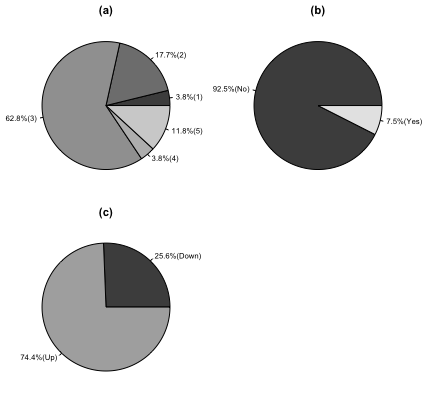
\includegraphics[scale=0.60]{figures/ds_distribution.png}
  \caption{Dataset distribution by severity level.}
\end{figure}


The graph (a) shows that of 8858 change requests, 3.8\% had severity 1(trivial); 17.7\% had severity 2(minor); 62.8\% had severity 3(major), 3.8\% had severity 4(critical), And 11.8\% had severity 5(blocker). The graph (b) shows that 92,5\% of them haven't changed their severities levels and 7,5\% have changed. And the last chart reveals that of the 7.5\% which changed their severity, 25,6\% reduced it, and 74,4\% increased it. We can note that dataset is clearly imbalanced.

\section{Findings and Discussions}

\subsection{RQ1: Is it possible to predict whether the change request severity level will shift during its lifecycle?(RQ1)}

The RQ1 is a simple binary problem or question whose answer is yes (positive class) or no (negative class). The Table \ref{tab:metrics_for_rq1} shows the performance of random forest to predict the answer to this question.

\begin{table}[!ht]
	\renewcommand{\arraystretch}{1.3}
	\caption{Random Forest Performance for RQ1.}
	\label{tab:metrics_for_rq1}
	\centering
	\begin{tabular}{|l|c|c|c|}
		\hline
		Accuracy & Precision & Recall & F-Measurement\\
		\hline
		94,128\% & 95,032\% & 1,000\% & 96,924\%\\
		\hline
	\end{tabular}
\end{table}


We tested the model with 3423(40\% of 8858) change requests: 3167 have changed their severity level, and 256 haven't changed their severity level. The Figure \ref{fig:rf_performance_for_q1} in terms of the amount of change requests whose predictions of severity level changes was correct or incorrect. We can note that the random forest performance was also 94,13\%.

\begin{figure}[!hbt]
  \label{fig:rf_performance_for_q1}
  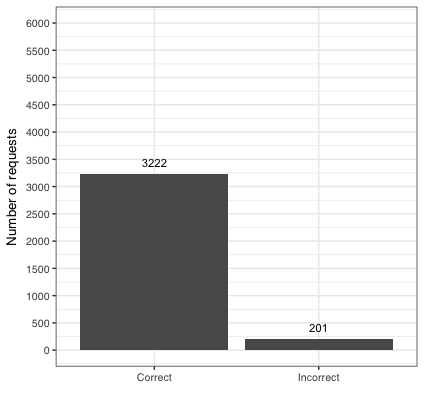
\includegraphics[scale=0.60]{figures/rf_performance_for_q1.png}
  \caption{Performance of Random Forest for RQ1.}
\end{figure}

\subsection{RQ2: Is it possible to predict whether the change request severity level will increase, decrease or remain the same during its lifecycle}

The RQ2 is a problem little harder than RQ1. It is a question with three responses classes related to severity: (-1) it was changed to down; (0)  it was maintained; and (1) it was changed to up.The Table \ref{tab:metrics_for_rq2} shows the performance of random forest to predict the answer to this question. 

\begin{table}[!ht]
	% increase table row spacing, adjust to taste
	\renewcommand{\arraystretch}{1.3}
	\caption{Evaluation metrics for RQ2.}
	\label{tab:metrics_for_rq2}
	\centering
	\begin{tabular}{|c|c|c|c|}
		\hline
		Class & Precision & Recall & F-Measurement\\
		\hline
		-1 & 6,15\% & 100,00\% & 11,59\%\\
		\hline
		0 & 100,00\% & 93,92\% & 96,86\%\\
		\hline
		1 & 22,11\% & 91,30\% & 35,59\%\\
		\hline\hline 
		Average & 42,75\% & 95,07\% & 48,02\% \\
		\hline 
	\end{tabular}
\end{table}

We tested the model with 3423(40\% of 8858) change requests: 3167 have changed their severity level, and 256 haven't changed their severity level. The Figure \ref{fig:rf_performance_for_q2} in terms of the amount of change requests whose predictions of severity level changes was correct or incorrect. We can note that the random forest performance was also 93,86\%.

\begin{figure}[!hbt]
   \label{fig:rf_performance_for_q2}
  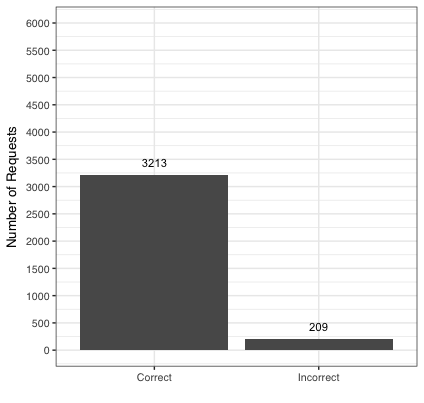
\includegraphics[scale=0.60]{figures/rf_performance_for_q2.png}
  \caption{Performance of Random Forest for RQ2.}
\end{figure}

\subsection{RQ3: Is it possible to predict the change request severity level at the end of its lifecycle?}

The RQ3 is a problem much harder than other two. It is a question with five responses classes related to severity: (1) trivial; (2) minor; (3) major; (4) critical; and (5) blocker. The Table \ref{tab:metrics_for_rq2} shows the performance of random forest to predict the answer to this question. 


\begin{table}[!ht]
	% increase table row spacing, adjust to taste
	\renewcommand{\arraystretch}{1.3}
	\caption{Evaluation metrics for RQ3.}
	\label{tab:metrics_for_rq3}
	\centering
	\begin{tabular}{|c|c|c|c|}
		\hline
		Class & Precision & Recall & F-Measurement\\
		\hline
		1 & 9,23\% & 100,00\% & 16,90\%\\
		\hline
		2 & 13,86\% & 77,77\% & 23,53\%\\
		\hline
		3 & 98,23\% & 67,34\% & 79,90\%\\
		\hline
		4 & 28,12\% & 100,00\% & 43,90\%\\
		\hline
		5 & 25,24\% & 80,95\% & 38,48\%\\
		\hline\hline 
		Average & 34,94\% & 85,21\% & 40,54\% \\
		\hline 
	\end{tabular}
\end{table}


We tested the model with 3423(40\% of 8858) change requests: 130 are trivial; 606 are minor; 2151 are major; 129 are critical; 405 are a blocker. The Figure \ref{fig:rf_performance_for_q3} shows three graphs. The graph (a) shows user range error in the assignment of severity level. The graph (b) shows the classifier error in the assignment of severity level. And the graph (c) compares de Predictor Error (PE) with User Error(UE) in terms of the amount of change requests whose predictions. We can note that the random forest performance was also 34,33\%.

\begin{figure}[!hbt]
  \center
  \label{fig:rf_performance_for_q3}
  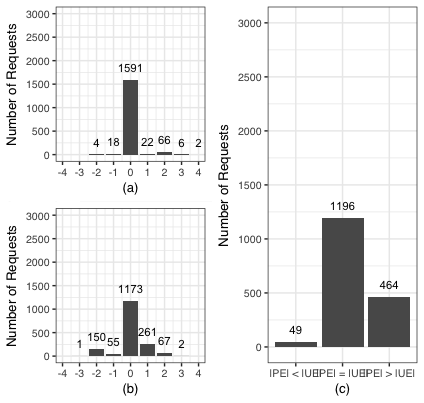
\includegraphics[scale=0.60]{figures/graphic_performance_q3_a.png}
  \caption{Performance of Random Forest for RQ3.}
\end{figure}


\section{Threats to Validity}
Runeson \cite{Runeson2009} recommends that threats to validity should be considered under four aspects: construct validity;  internal validity; external validity; and reliability.

\textbf{Construct validity}. Despite existing others metrics to evaluate classifiers\cite{Facelli2015}, which could be more suitable than precision, recall and F1-measure, we prefer to use them because they have been used satisfactorily in related works\cite{Menzies2008, Lamkanfi2010, Lamkanfi2011, ValdiviaGarcia2014}.


\textbf{Internal validity}. We assume that level of severity assignment by the user is correct and that there is an intimate relationship between it and the long description of the change request. This assumption finds echo or support in \cite{Lamkanfi2010, Tian2012}

\textbf{External validity}. We have considered one single repository and we have extracted 8858 change requests from it. Although we can't generalize the results to others, the characteristics presented by HADOOP repository, particularly regarding the balance of the data, are similars to those shown in the repositories studied\cite{Lamkanfi2010, Lamkanfi2011, Tian2012,ValdiviaGarcia2014}.

\textbf{Reliability}. The code developed in the Java language and the R language for preprocessing, training, testing and analysis of results have been carefully checked may contain bugs. To minimize this problem, we rely heavily on libraries offered by them such as XStream (the XML parser) and randomForest (a random forest implementation). 

\section{Conclusion and Future Work}
In this paper, we assess the Random Forest, a popular machine learning algorithm to CR severity level in imbalanced data scenario. We have considered the CR long description as the main factor to
this prediction. The features of machine learning were derived from
words(token) from this description. The results on a dataset consisting more than
8,000 CR from Hadoop have shown that random forest performed well to predict the severity level will change and whether severity will increase or decrease with reasonable accuracy, around 94,12\% and 93,86\% respectively. However, it has provided poor accuracy (around 67,29\%) to predict the final last severity level in imbalanced data scenario.

\section*{Acknowledgment}
This work has been carried out in the context of Ph.D program of  Computing Institute at State University of Campinas (UNICAMP), Brazil). Additional sponsoring by Permanent Professor Preparation Program(PPPP) of Pontifical Catholic University of Minas Gerais (PUC MG). 


% trigger a \newpage just before the given reference
% number - used to balance the columns on the last page
% adjust value as needed - may need to be readjusted if
% the document is modified later
%\IEEEtriggeratref{8}
% The "triggered" command can be changed if desired:
%\IEEEtriggercmd{\enlargethispage{-5in}}

% references section

% can use a bibliography generated by BibTeX as a .bbl file
% BibTeX documentation can be easily obtained at:
% http://www.ctan.org/tex-archive/biblio/bibtex/contrib/doc/
% The IEEEtran BibTeX style support page is at:
% http://www.michaelshell.org/tex/ieeetran/bibtex/
\bibliographystyle{IEEEtran}
% argument is your BibTeX string definitions and bibliography database(s)
\bibliography{references}
%
% <OR> manually copy in the resultant .bbl file
% set second argument of \begin to the number of references
% (used to reserve space for the reference number labels box)
%\begin{thebibliography}{1}
%\bibliographystyle{IEEEtran}

%\end{thebibliography}




% that's all folks
\end{document}


